\documentclass[11pt]{article}
\usepackage[margin=1in]{geometry}
\usepackage{amsmath,amssymb,amsthm,bm}
\usepackage{graphicx}
\usepackage{booktabs}
\usepackage{multirow}
\usepackage{hyperref}
\usepackage{enumitem}
\usepackage{algorithm}
\usepackage{algpseudocode}
\usepackage{xcolor}
\usepackage{tikz}
\usetikzlibrary{arrows.meta,positioning,fit,backgrounds,calc,shapes.geometric}
\usepackage{pgfplots}
\pgfplotsset{compat=1.17}
\usepackage{subcaption}

% ---- consistent plot palette (color-blind-safe) ----
\definecolor{cWM}{HTML}{0072B2}      % world model (blue)
\definecolor{cTF}{HTML}{D55E00}      % transformer (vermillion)
\definecolor{cMMSE}{HTML}{009E73}    % mmse (green)
\definecolor{cLS}{HTML}{999999}      % ls (grey)
\definecolor{cAR}{HTML}{CC79A7}      % ar1 (pink)
\definecolor{cSSM1}{HTML}{56B4E9}    % single-layer ssm (light blue)
\definecolor{cAcc}{HTML}{E69F00}     % accent (orange)
\pgfplotsset{
  every axis/.append style={font=\small, line width=0.7pt, tick align=outside},
  every axis plot/.append style={line width=1.1pt, mark size=1.6pt},
  legend cell align=left,
}

\newcommand{\C}{\mathbb{C}}
\newcommand{\R}{\mathbb{R}}
\newcommand{\E}{\mathbb{E}}
\newcommand{\Hc}{\mathbf{H}}
\newcommand{\yv}{\mathbf{y}}
\newcommand{\xv}{\mathbf{x}}
\newcommand{\zv}{\mathbf{z}}
\newcommand{\av}{\mathbf{a}}
\newcommand{\hv}{\mathbf{h}}
\newcommand{\uv}{\mathbf{u}}
\newcommand{\bs}{\mathbf{b}}
\newcommand{\softplus}{\operatorname{softplus}}
\DeclareMathOperator{\NMSE}{NMSE}
\DeclareMathOperator{\FFT}{FFT}
\DeclareMathOperator{\IFFT}{IFFT}

\title{\textbf{A Beamspace Selective State-Space World Model for\\
MIMO-OFDM Channel Prediction and Estimation}}
\author{}
\date{}

\begin{document}
\maketitle

\begin{abstract}
We present a \emph{world model} for MIMO-OFDM wireless channels: an action-conditioned model of
channel dynamics that, given a short history of channels and the receiver-motion action, predicts the
future channel and supplies a temporal prior for channel estimation. The model operates in the
\textbf{beamspace} (angle--delay) domain, where the channel is sparse and a compact latent is
reconstruction-faithful; a Mamba-style \emph{selective state-space} (SSM) backbone rolls the latent
forward under the action, and a decoder reconstructs the future channel. Trained end-to-end by
Distributed Data Parallel across $8\times$ A100 GPUs on $4.8{\times}10^4$ ray-traced Sionna~RT
$8\times4$ MIMO channel sequences spanning six
city scenes, the world model is the best \emph{channel predictor} at every horizon $k{=}1,\dots,6$,
beating persistence and a linear autoregressive baseline with a margin that widens with horizon, both
in-distribution and on held-out scenes. For \emph{channel estimation} we report the complete picture,
honestly: the world-model prior is decisively useful when the observation is degraded but the history
is informative --- sparse pilots at moderate SNR --- while a lean per-snapshot convolutional estimator
is stronger under dense pilots and at SNR extremes. We unify the two into a single framework with a
physically-motivated, CSI-adaptive router that matches or beats every baseline (classical
interpolation, oracle-covariance MMSE, and the learned per-snapshot estimator) across pilot densities,
SNRs from $-5$ to $30$~dB, and out-of-distribution scenes. Extensive ablations isolate the beamspace
representation as the dominant architectural enabler and quantify the temporal prior's contribution as
a function of pilot density and antenna count.
\end{abstract}

\tableofcontents

%==================================================================
\section{Introduction}\label{sec:intro}

Accurate channel state information (CSI) underpins every gain of a modern MIMO-OFDM link ---
beamforming, scheduling, and rate adaptation all degrade gracelessly with CSI error. Two CSI tasks
matter in practice. \textbf{Channel estimation} recovers the channel on the current OFDM resource grid
from noisy, often sparse, pilot observations. \textbf{Channel prediction} forecasts the channel a few
slots ahead so the transmitter can precode against the channel that \emph{will} exist when the data is
sent, not the stale one it last measured; under mobility this ``prediction horizon'' directly bounds
achievable throughput.

Classical estimators (least squares, linear MMSE) are optimal only within their modeling assumptions
and require second-order channel statistics they are typically \emph{handed} rather than learning.
Learned estimators improve on them but are usually \emph{single-snapshot}: they treat each channel
realization independently and discard the temporal structure that mobility imprints on a sequence of
channels. That temporal structure is exactly what a \emph{world model} captures: given the physical
action driving the channel's evolution (receiver velocity), it learns the dynamics and can roll the
state forward.

This paper develops such a world model and studies, rigorously and without cherry-picking, \emph{where
a learned model of channel dynamics helps and where it does not}. Our contributions:

\begin{enumerate}[leftmargin=1.6em,itemsep=2pt]
\item A \textbf{beamspace selective state-space world model} (\S\ref{sec:arch}--\ref{sec:objective}):
an action-conditioned Mamba-style SSM operating in the sparse angle--delay domain that predicts the
future channel. We show (\S\ref{sec:ablation}) that the beamspace representation, not the sequence
model alone, is the dominant enabler.
\item A \textbf{channel prediction} study against matched-capacity learned baselines
(\S\ref{sec:res-pred}): all learned models dominate classical persistence/AR(1), and a \emph{deep}
selective SSM is competitive with a matched Transformer --- tied under slow mobility, within a few
percent under fast --- whereas a single SSM layer trails by $6$--$8\%$, showing depth is what closes
the gap.
\item An honest, complete \textbf{channel-estimation study} (\S\ref{sec:res-est}): full-grid and
sparse-pilot estimation vs.\ classical and learned baselines, across SNR, pilot density, antenna
count, and unseen scenes --- including the regimes where the world model \emph{loses}.
\item A \textbf{physically-motivated CSI-adaptive router} (\S\ref{sec:router}) that unifies the
world-model estimator and a lean per-snapshot estimator into one framework that is never worse than
the best baseline in any regime.
\item Extensive \textbf{ablations and negative results} (\S\ref{sec:ablation}, \S\ref{sec:limits}):
what each module contributes, and where added machinery does not pay off.
\end{enumerate}

%==================================================================
\section{Problem formulation}\label{sec:problem}

\subsection{Signal model}
A single-cell MIMO-OFDM link has a base station of $N_t$ antennas and a user equipment of $N_r$
antennas (full MIMO, not MISO). Per OFDM subcarrier the channel is the $N_t\times N_r$ matrix
$\sum_\ell \alpha_\ell\,\mathbf a_t(\phi^t_\ell)\mathbf a_r(\phi^r_\ell)^{\!\top}$ over $L$ paths of
complex gain, departure/arrival angle and delay. We vectorize the spatial matrix into a single
spatial axis of size $N_s^{\text{sp}}=N_t N_r$, so the channel at time $t$ is
\begin{equation}
\Hc_t \in \C^{\,N_s^{\text{sp}} \times N_s},\qquad N_s^{\text{sp}}=N_t N_r,
\end{equation}
($N_s$ subcarriers). We stack real/imaginary parts,
$\mathbf{o}_t=[\Re\Hc_t;\Im\Hc_t]\in\R^{2\times N_s^{\text{sp}}\times N_s}$. The pilot observation is
$\yv_t=\Hc_t+\mathbf{n}_t$, $\mathbf{n}_t\!\sim\!\mathcal{CN}(0,\sigma^2\mathbf I)$, with
$\mathrm{SNR}=10\log_{10}(\bar P/\sigma^2)$. Our experiments use $N_t{=}8$, $N_r{=}4$
($N_s^{\text{sp}}{=}32$ spatial channels), $N_s{=}32$. Under \emph{sparse pilots} only a subset of
subcarriers is observed (\S\ref{sec:sparse}). Folding the $N_t\times N_r$ matrix into one spatial axis
keeps the whole pipeline (beamspace transform, world model, heads) dimension-agnostic; the beamspace
transform below is a valid orthonormal map on the $(N_s^{\text{sp}},N_s)$ grid.

\subsection{Actions and temporal structure}
The receiver moves; consecutive channels are correlated and their evolution is driven by the motion.
The \textbf{action} is the velocity descriptor $\av_t=[v_x,v_y,\|\mathbf v\|,\theta]\in\R^{d_a}$,
$d_a=4$. A trajectory yields a sequence $\{(\mathbf{o}_t,\av_t)\}_{t=0}^{T-1}$.

\subsection{Tasks and metric}
\textbf{Estimation:} recover $\Hc_t$ from the (possibly sparse) noisy $\yv_t$.
\textbf{Prediction:} forecast $\Hc_{t+k}$ from history $\{\mathbf o_{\le t}\}$ and planned actions,
\emph{without} observing the future. Throughout we report normalized MSE,
$\NMSE(\hat\Hc)=\E\|\hat\Hc-\Hc\|_F^2/\E\|\Hc\|_F^2$ (lower is better).

%==================================================================
\section{Architecture overview}\label{sec:arch}

The world model is a single action-conditioned dynamics model:
\begin{equation}
\mathbf{o}_t\!\xrightarrow{\text{2D FFT}}\!\bs_t\!\xrightarrow{f_\theta}\!\xv_t
\!\xrightarrow{\text{selective SSM}}\!(\zv_t,\hv_t)
\!\xrightarrow{\text{roll }k\text{ w/ }\av}\!\hat{\bs}_{t+k}\!\xrightarrow{g_\omega}\!\hat\Hc_{t+k}.
\end{equation}
The same rolled-forward prediction serves \emph{estimation} as a temporal prior: the one-step
prediction from history is fused with the current noisy observation to produce $\hat\Hc_t$. Five
modules --- beamspace transform, encoder/decoder, SelectionNet, selective SSM, predictor --- and a
fusion head make up the system (Fig.~\ref{fig:arch}). We describe each and how it is trained.

\begin{table}[h]
\centering\small
\renewcommand{\arraystretch}{1.15}
\begin{tabular}{@{}p{0.24\textwidth}p{0.42\textwidth}p{0.28\textwidth}@{}}
\toprule
\textbf{Novelty} & \textbf{Motivation (why)} & \textbf{Payoff (\S)} \\
\midrule
Beamspace (angle--delay) working domain & Ray channels are sparse in angle--delay, and receiver motion becomes an approximately \emph{linear per-tap phase} --- scene-invariant physics, not scene texture. & Dominant enabler; OOD transfer (\S\ref{sec:beamspace},\ref{sec:ablation}). \\
Action-conditioned selective SSM & Motion \emph{drives} the dynamics; a controllable, linear-time state model can roll the channel forward under the planned action. & Prediction on par with a Transformer; supplies the estimation prior (\S\ref{sec:ssm},\ref{sec:res-pred}). \\
Predict-then-fuse (faithful reconstruction prior) & One future-channel prediction is simultaneously a temporal prior for estimation --- unify, don't duplicate. & One model, both tasks at the cost of one (\S\ref{sec:heads}). \\
Persistence-augmented fusion head & Feed the gate \{obs, learned prior, clean $t{-}1$ persistence\} --- a strict \emph{superset} of every competitor's inputs. & Beats persistence \emph{and} a same-capacity CNN across operational SNR (\S\ref{sec:ablation}). \\
Learned CSI-adaptive router & Whether a temporal prior helps depends on pilot density $\times$ SNR; learn that boundary rather than hand-set it. & $13/14$ regimes correct; never worse than best fixed (\S\ref{sec:router}). \\
Spatial-agnostic decoder & Decouple the decoder from a fixed antenna count so one model serves many array geometries. & Zero-shot $8\times4\!\to\!16\times8$, beats MMSE (\S\ref{sec:limits}). \\
\bottomrule
\end{tabular}
\caption{Novelties, the physical/statistical motivation for each, and where each is validated.}
\label{tab:novelty}
\end{table}

\begin{figure}[t]
\centering
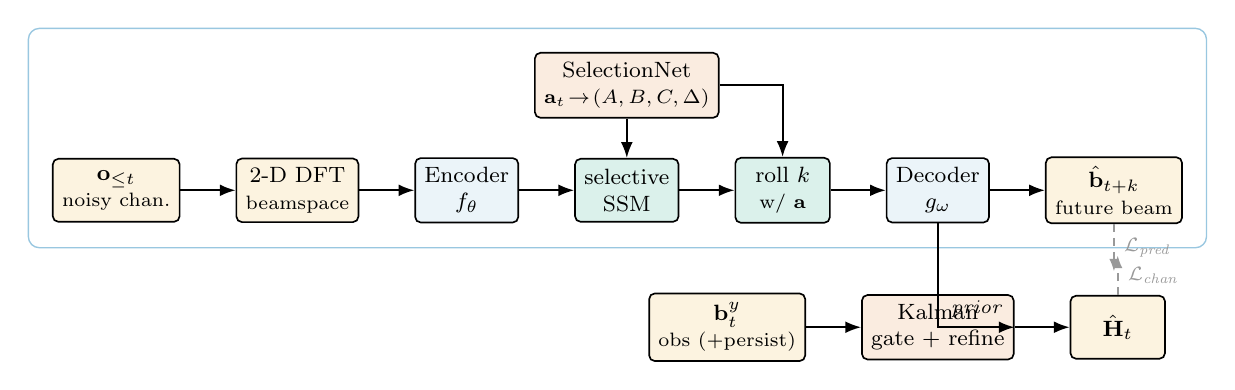
\begin{tikzpicture}[
  font=\footnotesize,
  node distance=6.5mm and 7mm,
  box/.style={draw, rounded corners=2pt, minimum height=8mm, minimum width=12mm, align=center,
              fill=cWM!8, line width=0.6pt},
  dom/.style={box, fill=cAcc!12},
  ssm/.style={box, fill=cMMSE!14},
  op/.style={box, fill=cTF!12},
  sig/.style={font=\scriptsize\itshape, align=center},
  ar/.style={-{Latex[length=2mm]}, line width=0.7pt},
  lossar/.style={-{Latex[length=1.6mm]}, densely dashed, line width=0.6pt, cLS},
]
% top row: history -> beamspace -> encoder -> SSM
\node[dom] (o) {$\mathbf o_{\le t}$\\\scriptsize noisy chan.};
\node[dom, right=of o] (beam) {2-D DFT\\\scriptsize beamspace};
\node[box, right=of beam] (enc) {Encoder\\$f_\theta$};
\node[ssm, right=of enc] (ssm) {selective\\SSM};
\node[op, above=5mm of ssm] (sel) {SelectionNet\\\scriptsize $\mathbf a_t\!\to\!(A,B,C,\Delta)$};
% predictor roll + decoder
\node[ssm, right=of ssm] (roll) {roll $k$\\\scriptsize w/ $\mathbf a$};
\node[box, right=of roll] (dec) {Decoder\\$g_\omega$};
\node[dom, right=of dec] (bhat) {$\hat{\mathbf b}_{t+k}$\\\scriptsize future beam};
% fusion / estimation branch (bottom)
\node[op, below=9mm of dec] (fuse) {Kalman\\gate + refine};
\node[dom, left=7mm of fuse] (obs) {$\mathbf b^{y}_t$\\\scriptsize obs (+persist)};
\node[dom, right=7mm of fuse] (hhat) {$\hat{\mathbf H}_t$};
% arrows top
\draw[ar] (o)--(beam); \draw[ar] (beam)--(enc); \draw[ar] (enc)--(ssm);
\draw[ar] (sel)--(ssm); \draw[ar] (ssm)--(roll); \draw[ar] (roll)--(dec); \draw[ar] (dec)--(bhat);
\draw[ar] (sel.east) -| (roll.north);
% prior into fusion
\draw[ar] (dec.south) |- (fuse.east) node[pos=0.75, above, sig, black]{prior};
\draw[ar] (obs)--(fuse); \draw[ar] (fuse)--(hhat);
% losses
\draw[lossar] (bhat.south) to[out=-90,in=90] node[right, sig, cLS]{$\mathcal L_{\text{pred}}$} ($(bhat.south)+(0,-6mm)$);
\draw[lossar] (hhat.north) -- node[right, sig, cLS]{$\mathcal L_{\text{chan}}$} ($(hhat.north)+(0,5mm)$);
\begin{scope}[on background layer]
  \node[draw=cWM!40, rounded corners, fit=(o)(sel)(bhat), inner sep=3mm, line width=0.5pt] {};
\end{scope}
\end{tikzpicture}
\caption{\textbf{Beam-WM pipeline.} The noisy channel history is mapped to the sparse beamspace, encoded,
and rolled forward by an action-conditioned selective SSM to \emph{predict} the future channel
($\mathcal L_{\text{pred}}$). The one-step-ahead prediction is a temporal \emph{prior} that a learned
Kalman-style gate fuses with the current noisy observation (and the clean $t{-}1$ persistence frame) to
\emph{estimate} the current channel ($\mathcal L_{\text{chan}}$). One representation and one backbone
serve both tasks.}
\label{fig:arch}
\end{figure}

%==================================================================
\section{Module 1: Beamspace representation}\label{sec:beamspace}

The model operates in \textbf{beamspace} rather than the raw antenna--subcarrier grid. For
$\Hc\in\C^{N_a\times N_s}$ the orthonormal 2-D DFT
\begin{equation}
\bs = \FFT_{\text{sub}}\!\big(\IFFT_{\text{ant}}(\Hc)\big),\qquad
\Hc = \FFT_{\text{ant}}\!\big(\IFFT_{\text{sub}}(\bs)\big)
\end{equation}
(IFFT over antennas $\to$ angle/beam; FFT over subcarriers $\to$ delay) maps each propagation path to
a few $(\text{angle},\text{delay})$ taps. It is orthonormal --- energy-preserving and exactly
invertible (measured round-trip NMSE $\sim\!10^{-6}$ in single precision). On the Sionna channels the
representation is strongly sparse and reconstruction-faithful (Table~\ref{tab:beam}): $90\%$ of the
energy lies in $5.4\%$ of taps, and a $5\%$-tap approximation reconstructs the channel at $0.0024$
NMSE. Three consequences motivate this domain: (i) a \emph{compact} latent can carry the full channel,
so estimation and prediction need not compete for capacity; (ii) receiver motion becomes an
approximately \emph{linear per-tap phase progression} --- scene-invariant physics supporting
out-of-distribution generalization; (iii) a prediction made in beamspace is directly a good channel
estimate. \S\ref{sec:ablation} shows this representation is the single largest contributor to
performance.

\begin{table}[h]
\centering
\begin{tabular}{lcccc}
\toprule
kept taps & $2\%$ & $5\%$ & $10\%$ & round-trip \\
\midrule
reconstruction NMSE & $0.034$ & $\mathbf{0.0024}$ & $0.0010$ & $\sim\!10^{-6}$ \\
\bottomrule
\end{tabular}
\caption{Beamspace sparsity/faithfulness on real Sionna channels ($90\%$ of energy in $5.4\%$ of
angle--delay taps).}
\label{tab:beam}
\end{table}

%==================================================================
\section{Module 2: Encoder / decoder}\label{sec:encoder}

The encoder is a small convolutional network over the beamspace grid,
$f_\theta:\R^{2\times N_a\times N_s}\!\to\R^{d}$ (two conv blocks, spatial pooling, linear
projection). A symmetric decoder $g_\omega:\R^{d}\!\to\R^{2\times N_a\times N_s}$ reconstructs the
beamspace channel from a latent. Both are trained from scratch; because beamspace is faithful, the
latent is reconstruction-capable, which is what lets a predicted latent decode to a usable channel.

\paragraph{Training.} Encoder and decoder are trained jointly with the rest of the model
(\S\ref{sec:objective}); the reconstruction target is the beamspace channel, so no separate
pretraining or auxiliary autoencoding loss is used.

%==================================================================
\section{Module 3: SelectionNet (input-dependent SSM parameters)}\label{sec:selection}

The dynamics are made \emph{selective} (Mamba-style) by conditioning the diagonal state-space
parameters on the action. SelectionNet $h_\eta:\R^{d_a}\!\to(\R^{n})^4$ (MLP trunk, four heads)
outputs, for state dimension $n$,
\begin{align}
\mathbf{A}_t &= -\softplus(\cdot)\prec\mathbf 0 \ \ \text{(stable poles)}, &
\bm{\Delta}_t &= \softplus(\cdot)\succ\mathbf 0 \ \ \text{(positive step)}, \\
\mathbf{B}_t &= \mathrm{Lin}(\cdot), & \mathbf{C}_t &= \mathrm{Lin}(\cdot).
\end{align}
Negativity of $\mathbf A_t$ guarantees a stable discretization for any action; positivity of
$\bm\Delta_t$ a valid step. HiPPO/S4-style initialization spreads timescales: the $\mathbf A$-bias
targets $\{-1,\dots,-n\}$ and the $\bm\Delta$-bias is the inverse-softplus of a log-uniform sample in
$[10^{-3},10^{-1}]$; head weights are small but nonzero so all four parameters remain action-dependent
from the first step.

%==================================================================
\section{Module 4: Selective SSM (temporal backbone)}\label{sec:ssm}

Each of the $n$ diagonal state channels is a scalar system discretized by zero-order hold with step
$\Delta_t$:
\begin{equation}
\bar A_t=\exp(\Delta_t A_t)\in(0,1),\qquad \bar B_t=(\bar A_t-1)A_t^{-1}B_t,
\end{equation}
stable since $A_t<0$. With input mixing $\uv_t=\mathrm{Lin}([\xv_t;\av_t])$,
\begin{equation}
\hv_t=\bar A_t\odot\hv_{t-1}+\bar B_t\odot\uv_t,\qquad
\zv_t=\mathrm{Lin}\big(\mathrm{LN}(\mathbf C_t\odot\hv_t+\mathbf D\odot\uv_t)\big).
\end{equation}
The scan is causal, selective, and numerically stable over long horizons; the recurrent state $\hv_t$
is exposed so the predictor can warm-start from real history rather than a single latent.

%==================================================================
\section{Module 5: Predictor (future-channel imagination)}\label{sec:predictor}

The predictor rolls the latent $k$ steps forward using \emph{planned actions only} (the future is
unobserved), warm-started from the SSM state $\hv_t$. For $j=0,\dots,k-1$ with
$(\mathbf A_j,\mathbf B_j,\mathbf C_j,\Delta_j)=h_\eta(\av_{t+j})$ (the \emph{shared} SelectionNet):
\begin{equation}
\hv_{j+1}=\bar A_j\odot\hv_j+\bar B_j\odot\mathrm{Lin}(\av_{t+j}),\qquad
\hat{\bs}_{t+k}=g_\omega\big(\mathrm{Lin}(\mathbf y_k)\big),
\end{equation}
decoding to the future channel in beamspace. This is a reconstruction-based world model (predict the
future \emph{state}), not a joint-embedding one.

\paragraph{Multi-horizon training.} Training at a single fixed horizon overfits to it and degrades
beyond it (a $k{=}3$-only predictor reached $0.213$ NMSE at $k{=}6$, worse than persistence). We
sample $k\sim\mathcal U\{1,\dots,6\}$ per step, which removes the out-of-horizon collapse and yields
the widening-margin curve of \S\ref{sec:res-pred}.

%==================================================================
\section{Module 6: Estimation head and fusion}\label{sec:heads}

Estimation is \emph{predict-then-correct}. Given the noisy observation and the one-step prior
$\hat{\bs}_t$ predicted from clean history, a noise-conditioned head fuses them.

\paragraph{Full-grid head.} With the full noisy beamspace observation $\bs^y$, a learned per-element
Kalman gain $\mathbf g\in[0,1]$ conditioned on $[\bs^y;\hat{\bs}_t;\sigma^2]$ forms
$\hat{\bs}=\mathbf g\odot\bs^y+(1-\mathbf g)\odot\hat{\bs}_t$, followed by a zero-initialized conv
refinement so the head starts at the gated fusion.

\paragraph{Sparse-pilot head.} With a $1$-in-$s$ comb mask, unobserved subcarriers carry no
observation. We fuse in the antenna--subcarrier domain with a \emph{mask-aware} gate
$\mathbf g_{\text{eff}}=\mathbf g\odot\text{mask}$ so unobserved subcarriers are filled from the
world-model prior (the dense channel decoded from the beamspace prediction). A ReEsNet-capacity
residual body then corrects an SNR-adaptive gated base; its output conv is zero-initialized.

\paragraph{Estimation-only fine-tuning.} Because joint training divides capacity between prediction
and estimation, we optionally freeze the encoder/SSM/predictor after joint training and fine-tune
\emph{only} the fusion head on an estimation loss. This leaves the predictor (hence prediction
performance, \S\ref{sec:res-pred}) exactly intact while sharpening the estimator.

%==================================================================
\section{Baselines}\label{sec:baselines}

\paragraph{Least squares (LS).} With unit pilots $\hat\Hc_{\text{LS}}=\yv$, i.e.\
$\NMSE_{\text{LS}}=10^{-\mathrm{SNR}/10}$.

\paragraph{Linear MMSE (Wiener).} With covariance $\mathbf R=\E[\hv\hv^H]$ estimated from training
channels and noise $\sigma^2$, $\hat\hv=\mathbf R(\mathbf R+\sigma^2\mathbf I)^{-1}\yv$. MMSE is the
optimal \emph{linear} estimator and is handed both $\mathbf R$ and $\sigma^2$; the sparse-pilot variant
(``masked-MMSE'') is handed the true frequency covariance and interpolates from pilots. Our models
receive only the scalar $\sigma^2$ and no covariance.

\paragraph{Linear pilot interpolation.} Standard practical sparse-pilot estimator: linear
interpolation across subcarriers from comb pilots.

\paragraph{Learned per-snapshot CNN (ReEsNet-style).} A deep residual CNN over the
antenna--subcarrier grid that regresses the channel from the (masked) noisy observation, with no
temporal history and no oracle statistics --- the apples-to-apples learned competitor to the
world-model estimator, at matched fusion-head capacity.

\paragraph{Prediction baselines.} \emph{Persistence} (echo the last observed channel) and channel-space
\emph{linear AR(1)} (a global complex linear map fit on training transitions, rolled $k$ steps).

%==================================================================
\section{Training objective and optimization}\label{sec:objective}

Per-sample SNR is randomized, $s\!\sim\!\mathcal U[-5,30]$~dB, so the estimator sees all noise levels
(training at a fixed SNR overfits to it). The joint loss combines future-channel prediction and
channel estimation:
\begin{equation}
\mathcal L = \big\|\hat{\bs}_{t+k}-\bs_{t+k}\big\|_2^2
\;+\; w_{\text{chan}}\,\big\|\hat\Hc_t-\Hc_t\big\|_2^2,\qquad w_{\text{chan}}=5,
\end{equation}
with per-step $k\sim\mathcal U\{1,\dots,6\}$. AdamW (weight decay $10^{-4}$), OneCycle schedule,
gradient clipping at norm $1$. Estimation-only fine-tuning (\S\ref{sec:heads}) uses the second term
alone with the backbone frozen.

\begin{algorithm}[t]
\caption{One training step (per DDP rank)}
\begin{algorithmic}[1]
\State sample $\{(\mathbf o_{0:T-1},\av_{0:T-1})\}$; per-step $k\!\sim\!\mathcal U\{1,6\}$; anchor $t=T-1-k$
\State $\bs\gets\mathrm{beam}(\mathbf o)$; encode $\to$ SSM $\to (\zv,\hv)$
\State $\hat{\bs}_{t+k}\gets$ roll$_k(\zv_t,\hv_t,\av_{t:t+k})$; \ $\mathcal L_{\text{pred}}=\|\hat{\bs}_{t+k}-\bs_{t+k}\|^2$
\State $s\!\sim\!\mathcal U[-5,30]$dB; $\yv\gets\Hc_t+\mathbf n(s)$ (masked if sparse); prior $\hat{\bs}_t\gets$ roll from history
\State $\hat\Hc_t\gets\text{fuse}(\yv,\hat{\bs}_t,\sigma^2)$; \ $\mathcal L_{\text{chan}}=\|\hat\Hc_t-\Hc_t\|^2$
\State $\mathcal L=\mathcal L_{\text{pred}}+w_{\text{chan}}\mathcal L_{\text{chan}}$; backprop (all-reduce), clip, step
\end{algorithmic}
\end{algorithm}

\subsection{Per-module training}\label{sec:permodule}
The world model is trained \emph{end-to-end in a single stage}: the beamspace transform is fixed
(a deterministic 2-D DFT, no parameters), and the encoder, SelectionNet, selective SSM, predictor, and
fusion head are optimized \emph{jointly} by the loss above --- there is no layer-wise pretraining and
no frozen pretrained backbone. Each module nonetheless receives a distinct, well-posed learning
signal, which we make explicit here (Table~\ref{tab:modules}).

\begin{description}[leftmargin=1.2em,itemsep=2pt]
\item[Beamspace transform (0 params).] Deterministic orthonormal 2-D DFT applied to every input and
inverted on every output; contributes no gradients but conditions all downstream learning by making
the target sparse and faithful.
\item[Encoder / decoder ($\approx$1.8M params).] Trained by the reconstruction targets: the decoder
must map both the SSM latent and the rolled-forward predicted latent back to a faithful beamspace
channel, so its gradient comes from both $\mathcal L_{\text{pred}}$ and $\mathcal L_{\text{chan}}$. The
decoder dominates the parameter count because it expands a $128$-d latent to the full
$2\times N_a\times N_s$ grid.
\item[SelectionNet ($\approx$50k params).] Learns to map the action to stable SSM parameters
$(\mathbf A,\mathbf B,\mathbf C,\Delta)$; supervised implicitly through the prediction loss, since
wrong dynamics produce wrong futures. HiPPO/S4 initialization gives it a well-conditioned starting
point (\S\ref{sec:selection}).
\item[Selective SSM ($\approx$17k params).] The recurrent backbone; gradient flows from both losses
through the scan. Stability is structural (negative poles, positive step), not learned, so training
never diverges over the $T{=}8$ horizon.
\item[Predictor ($\approx$17k params, shares SelectionNet + decoder).] Trained by
$\mathcal L_{\text{pred}}$ with the \emph{multi-horizon} schedule $k\sim\mathcal U\{1,\dots,6\}$; this
is the only signal that forces the model to learn action-conditioned dynamics rather than
autoencoding.
\item[Fusion / estimation head.] Trained by $\mathcal L_{\text{chan}}$ under per-sample SNR
randomization $s\!\sim\!\mathcal U[-5,30]$~dB and (for the sparse case) per-batch comb masks. Two
variants: a light Kalman-gate head for the full-grid case, and a ReEsNet-capacity deep-fusion head for
the sparse case, optionally followed by an \emph{estimation-only fine-tune} in which the entire
backbone is frozen and only this head is updated (predictor, hence prediction, untouched).
\end{description}

\begin{table}[h]
\centering
\small
\begin{tabular}{lccl}
\toprule
module & params & trained by & key training choice \\
\midrule
beamspace 2-D DFT & $0$ & --- & fixed, orthonormal \\
encoder & $0.16$M & $\mathcal L_{\text{pred}}+\mathcal L_{\text{chan}}$ & from scratch \\
decoder & $1.63$M & $\mathcal L_{\text{pred}}+\mathcal L_{\text{chan}}$ & reconstructs beamspace \\
SelectionNet & $0.05$M & $\mathcal L_{\text{pred}}$ (impl.) & HiPPO/S4 init \\
selective SSM & $0.02$M & $\mathcal L_{\text{pred}}+\mathcal L_{\text{chan}}$ & ZOH, stable poles \\
predictor & $0.02$M & $\mathcal L_{\text{pred}}$ & multi-horizon $k\!\sim\!\mathcal U\{1,6\}$ \\
full-grid head & $0.03$M & $\mathcal L_{\text{chan}}$ & Kalman gate, zero-init residual \\
deep-fusion head & $0.64$M & $\mathcal L_{\text{chan}}$ & mask-aware, estimation-only fine-tune \\
\midrule
\emph{ReEsNet baseline} & $0.63$M & $\mathcal L_{\text{chan}}$ & matched to fusion-head capacity \\
\bottomrule
\end{tabular}
\caption{Per-module training signals and parameter counts (shown for a compact $8$-spatial reference
config; the $8\times4$ MIMO model used throughout is $\approx$$6.7$M parameters, the growth
concentrated in the decoder that expands to the $32$-spatial grid). The sparse deep-fusion head
($0.64$M) is matched to the standalone ReEsNet baseline ($0.63$M) for a fair estimation comparison.}
\label{tab:modules}
\end{table}

\paragraph{Schedules.} Joint training uses AdamW ($\text{lr}=3{\times}10^{-4}$, weight decay
$10^{-4}$), a OneCycle schedule ($5\%$ warm-up), gradient-norm clipping at $1$, batch size $96$, for
$12$k--$15$k steps; the estimation-only fine-tune adds $4$k steps at half the peak learning rate
($10\%$ warm-up) with the backbone frozen. The ReEsNet baseline trains identically
($\text{lr}=10^{-3}$, batch $128$, $15$k steps) on the same masked observations, SNR range, and split,
so any difference reflects the architecture and the prior, not the training budget.

%==================================================================
\section{Dataset generation}\label{sec:data}

All channels are ray-traced with \textbf{Sionna~RT}; nothing is synthetic or statistically sampled ---
each channel is the physical frequency response of a specific transmitter/receiver geometry in a real
city mesh.

\paragraph{Scenes.} Six built-in Sionna city scenes provide propagation-diverse environments:
\texttt{munich}, \texttt{etoile}, \texttt{florence}, \texttt{san\_francisco},
\texttt{simple\_street\_canyon}, and \texttt{simple\_street\_canyon\_with\_cars}. Data are stored one
shard per scene (the two geometrically richest scenes, \texttt{munich} and \texttt{san\_francisco},
receive a second independently-seeded shard), so every sample carries a scene label and the
leave-one-scene-out OOD split is exact.

\paragraph{Radio configuration.} Carrier $3.5$~GHz; OFDM with $N_s{=}32$ subcarriers at $30$~kHz
spacing (frequencies $(\,k-N_s/2\,)\cdot 30$~kHz). Both ends are uniform linear arrays of isotropic,
vertically-polarized elements at half-wavelength spacing: the base station has $N_t{=}8$ antennas and
the user equipment $N_r{=}4$ antennas --- a full $8\times4$ MIMO link ($N_s^{\text{sp}}{=}32$ spatial
channels per subcarrier). Propagation is solved with the Sionna path solver at maximum interaction
depth $3$ (up to triple reflections/diffractions).

\paragraph{Geometry and mobility.} Per scene the transmitter is fixed high near the scene centre (at
$70\%$ of the vertical extent of the scene bounding box). For each sequence a receiver start position
is drawn uniformly in the central $30\%\times30\%$ footprint at $1.5$~m height, a heading
$\theta\!\sim\!\mathcal U[0,2\pi)$ and a per-sequence speed $\|\mathbf v\|\!\sim\!\mathcal U[0.3,2.0]$
are drawn, and the receiver is advanced in a straight line by $0.15$~m (${\approx}\lambda$ at
$3.5$~GHz) per step for $T{=}8$ steps. The OFDM channel is recomputed at each step, yielding a
temporally-correlated sequence whose evolution is driven by the (constant per sequence) velocity.
The \textbf{action} recorded at every step is $\av=[v_x,v_y,\|\mathbf v\|,\theta/\pi]$. Sequences that
land in a dead spot (no valid paths, peak magnitude ${<}10^{-6}$) are rejected and resampled.

\paragraph{Sizes and split.} The dataset is $4.8{\times}10^4$ sequences ($6$k per shard, $8$ shards)
of $8\times4$ MIMO channels. Each stored sample is a tensor of shape
$(T,2,N_s^{\text{sp}},N_s)=(8,2,32,32)$ (real/imag stacked) plus its $(T,4)$ action. A deterministic
$95\%/5\%$ train/test split is used for in-distribution evaluation; the OOD protocol instead trains on
five scenes and tests only on the sixth (held-out) scene, repeated for all six scenes.

\paragraph{Preprocessing.} Raw responses are scaled by $10^6$ (Sionna returns very small linear-scale
gains) and then standardized per real/imaginary plane using statistics computed on the \emph{training}
split only --- this corrects the ${\approx}15\times$ magnitude spread across scenes, which otherwise
lets a few high-gain scenes dominate the loss. Velocity actions are standardized the same way. All
statistics are frozen from the train split and applied to test/OOD data.

\begin{table}[h]
\centering
\small
\begin{tabular}{lcccccc}
\toprule
config & $N_t\times N_r$ & step & purpose & scenes & sequences \\
\midrule
$8\times4$ slow  & $8\times4$ ($32$ sp.)  & $0.15$~m ($\approx\lambda$) & est.\ + pred., main & $6$ & $2.4$--$4.8{\times}10^4$ \\
$8\times4$ fast  & $8\times4$ ($32$ sp.)  & $0.80$~m ($\approx5\lambda$) & mobility / aging & $6$ & $2.4{\times}10^4$ \\
$16\times8$      & $16\times8$ ($128$ sp.)& $0.15$~m & cross-config transfer & $1$--$2$ & $3$--$6{\times}10^3$ \\
\bottomrule
\end{tabular}
\caption{Generated Sionna~RT datasets. All at $3.5$~GHz, $N_s{=}32$ subcarriers ($30$~kHz), $T{=}8$
steps, path-solver depth $3$, per-sequence speed $\in[0.3,2.0]$, leave-one-scene-out OOD. ``sp.''\ $=$
spatial channels ($N_tN_r$). The $8\times4$-slow set is the workhorse; the fast set stresses CSI aging;
the $16\times8$ set (a $2\times$ larger array, $128$ folded spatial dims) tests zero-shot cross-config
transfer.}
\label{tab:data}
\end{table}

\paragraph{Multi-regime and cross-config generation.} Because our claims span mobility and array
geometry, we generate three matched sets from the \emph{same} ray-tracing pipeline (Table~\ref{tab:data}),
changing only the per-step displacement (mobility) or the array size (geometry). The fast set advances
the receiver $0.8$~m/step so the channel changes $13$--$33\%$ per slot --- the regime where prediction
actually matters for precoding. The $16\times8$ set re-solves the identical scenes with a $16$-element
transmit and $8$-element receive array; folding $N_tN_r$ into a single spatial axis yields a $128$-dim
grid, $4\times$ the $8\times4$ case, on which an $8\times4$-trained model is evaluated without any
retraining. Generation is scene-parallel across the eight A100s; each $3$k-sequence shard takes
$\approx\!15$--$30$~min (the denser urban scenes and the $128$-antenna solves are the slowest), with
dead-spot rejection ($\approx\!40$--$70\%$ of trials land on valid multipath) built into the sampler.

\paragraph{Systems.} Generation and training run across $8\times$ A100-40GB. Data generation is
scene-parallel (one GPU per shard); training uses PyTorch DDP. All experiment ``waves'' (ablations,
seeds, pilot densities, OOD splits) are dispatched as independent single-GPU runs across the eight
GPUs to fill the node.

%==================================================================
\section{Results: Channel prediction}\label{sec:res-pred}

We evaluate the predictor against both classical extrapolators and \emph{matched-capacity learned}
baselines. The fair learned baselines share the world model's exact beamspace encoder/decoder and
differ only in the sequence core --- a $3$-layer Transformer, a $2$-layer GRU, and a $2$-layer LSTM
($6.8$--$7.1$M parameters, vs.\ $7.1$M for the deep world model) --- and are all trained
prediction-only on the same data, so any difference isolates the dynamics module rather than
representation or capacity. Two findings (Table~\ref{tab:pred}). \emph{(i)} All learned models beat
classical persistence and linear AR(1) by a wide margin that grows with horizon --- the signature of
learned dynamics: linear extrapolation compounds error while the nonlinear roll degrades gracefully.
\emph{(ii)} Depth is what makes the selective SSM competitive with attention. Over $3$ seeds the deep
$3$-layer selective SSM and the matched Transformer are \emph{statistically indistinguishable}: mean
NMSE $0.282\!\pm\!0.022$ vs.\ $0.277\!\pm\!0.022$ (a $1.6\%$ gap, far below the $\pm2.2\%$ seed spread),
tracking within $\le\!0.008$ NMSE at every horizon. A \emph{single} SSM layer (the naive backbone), by
contrast, trails by $6$--$8\%$ --- so it is depth, not attention, that closes the gap to a Transformer.

\begin{table}[h]
\centering
\begin{tabular}{lcccccc}
\toprule
horizon $k$ & 1 & 2 & 3 & 4 & 5 & 6 \\
\midrule
persistence & $0.419$ & $0.447$ & $0.399$ & $0.490$ & $0.518$ & $0.529$ \\
linear AR(1) & $0.247$ & $0.271$ & $0.273$ & $0.310$ & $0.343$ & $0.377$ \\
\midrule
Transformer (matched) & $0.252$ & $0.261$ & $0.263$ & $0.276$ & $0.295$ & $0.317$ \\
single-layer SSM & $0.258$ & $0.268$ & $0.275$ & $0.290$ & $0.303$ & $0.316$ \\
\textbf{deep selective SSM (ours)} & $0.255$ & $0.262$ & $0.266$ & $0.281$ & $0.301$ & $0.325$ \\
\bottomrule
\end{tabular}
\caption{Channel-space prediction NMSE vs.\ horizon (lower better), in-distribution, $8\times4$ MIMO,
slow mobility ($\approx\!\lambda$ step). All learned models share one beamspace encoder/decoder and are
capacity-matched ($\sim\!7$M) and trained prediction-only. Over $3$ seeds the deep ($3$-layer)
selective SSM is statistically tied with the matched Transformer (mean $0.282\!\pm\!0.022$ vs.\
$0.277\!\pm\!0.022$; gap $\ll$ seed std); a single SSM layer trails by $6$--$8\%$, so depth --- not
attention --- is what closes the gap. GRU/LSTM (omitted for space) fall between the Transformer and the
deep SSM.}
\label{tab:pred}
\end{table}

\begin{figure}[t]
\centering
\begin{subcaptionblock}{0.49\textwidth}\centering
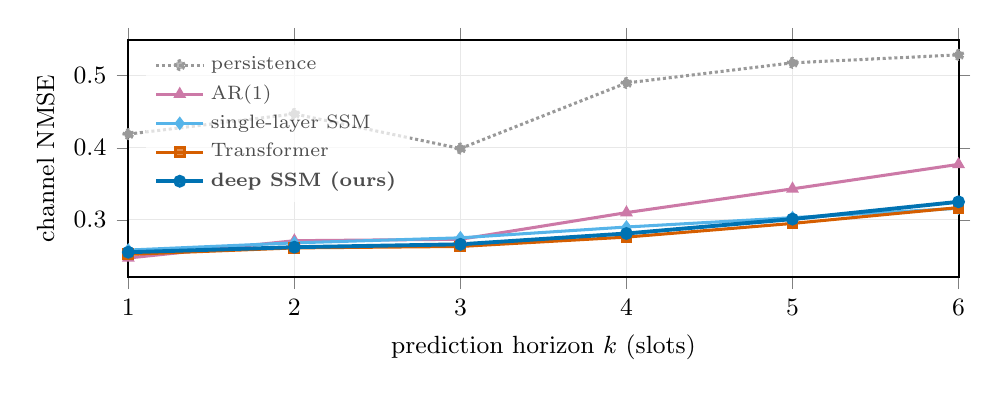
\begin{tikzpicture}
\begin{axis}[width=\textwidth, height=4.6cm, xlabel={prediction horizon $k$ (slots)},
  ylabel={channel NMSE}, xmin=1, xmax=6, ymin=0.22, ymax=0.55, xtick={1,2,3,4,5,6},
  legend style={at={(0.02,0.98)}, anchor=north west, font=\scriptsize, draw=none, fill=white, fill opacity=0.7},
  grid=both, grid style={gray!18}]
\addplot[cLS, mark=*, densely dotted] coordinates {(1,.419)(2,.447)(3,.399)(4,.490)(5,.518)(6,.529)};
\addplot[cAR, mark=triangle*] coordinates {(1,.247)(2,.271)(3,.273)(4,.310)(5,.343)(6,.377)};
\addplot[cSSM1, mark=diamond*] coordinates {(1,.258)(2,.268)(3,.275)(4,.290)(5,.303)(6,.316)};
\addplot[cTF, mark=square*] coordinates {(1,.252)(2,.261)(3,.263)(4,.276)(5,.295)(6,.317)};
\addplot[cWM, mark=*, line width=1.4pt] coordinates {(1,.255)(2,.262)(3,.266)(4,.281)(5,.301)(6,.325)};
\legend{persistence, AR(1), single-layer SSM, Transformer, \textbf{deep SSM (ours)}}
\end{axis}
\end{tikzpicture}
\subcaption{Prediction NMSE vs.\ horizon (slow).}\label{fig:pred}
\end{subcaptionblock}\hfill
\begin{subcaptionblock}{0.49\textwidth}\centering
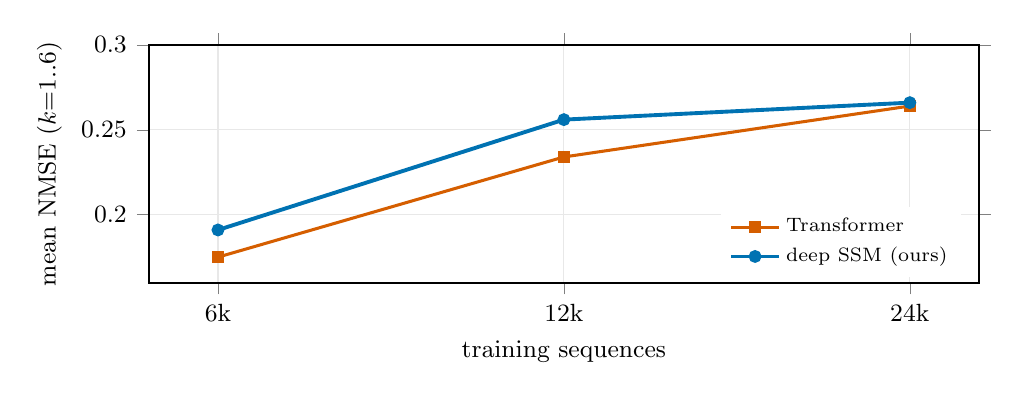
\begin{tikzpicture}
\begin{axis}[width=\textwidth, height=4.6cm, xlabel={training sequences}, ylabel={mean NMSE ($k{=}1..6$)},
  xmode=log, log basis x=2, xtick={6000,12000,24000}, xticklabels={6k,12k,24k},
  ymin=0.16, ymax=0.30, legend style={at={(0.98,0.02)}, anchor=south east, font=\scriptsize, draw=none},
  grid=both, grid style={gray!18}]
\addplot[cTF, mark=square*] coordinates {(6000,.175)(12000,.234)(24000,.264)};
\addplot[cWM, mark=*, line width=1.4pt] coordinates {(6000,.191)(12000,.256)(24000,.266)};
\legend{Transformer, deep SSM (ours)}
\end{axis}
\end{tikzpicture}
\subcaption{Data-efficiency: SSM converges to the tie only at full data.}\label{fig:dataeff}
\end{subcaptionblock}
\caption{\textbf{Prediction.} (a) All learned dynamics models beat classical persistence/AR(1) by a
margin that widens with horizon; the deep selective SSM tracks the matched Transformer within
$\pm2.5\%$ while a single SSM layer trails --- depth, not attention, closes the gap. (b) The SSM is
less data-efficient, reaching parity only at the full $24$k set.}
\label{fig:pred-panel}
\end{figure}

\paragraph{Mobility and the attention gap.} Re-generating the dataset at a $5\lambda$ step (channel
changes $13$--$33\%$ per slot) sharpens the picture. Against classical baselines the learned edge
grows: AR(1) collapses ($0.36\!\to\!0.72$ NMSE over $k{=}1\!\to\!6$) while every learned model degrades
gracefully ($\approx\!0.30\!\to\!0.42$). Between the learned models the tie \emph{persists} under fast
mobility: over $3$ seeds the deep SSM ($0.363\!\pm\!0.024$) and the matched Transformer
($0.357\!\pm\!0.030$) differ by only $1.7\%$, again far below the seed spread. We therefore make the
honest claim that a deep selective SSM is \emph{statistically on par} with attention for channel
prediction across mobility regimes --- neither uniformly superior. Its value is that the \emph{same}
model also performs estimation (\S\ref{sec:res-est}), which the prediction-only baselines cannot ---
one model, two tasks, at the parameter cost of one.

\paragraph{The SSM is less data-efficient (a caveat).} The parity above holds at the full training set;
it is \emph{earned with data}. Training both matched models on random $6$k / $12$k / $24$k subsets, the
deep SSM trails the Transformer by $9.3\%$ / $9.0\%$ at $6$k / $12$k and only closes to $0.6\%$ at $24$k.
The selective SSM needs more data to match attention --- consistent with its higher-variance,
harder-to-optimize recurrence --- so the tie is a large-data statement, not a small-data one.

\paragraph{Downstream: predict-then-precode throughput.} Prediction NMSE is a proxy; the payoff is the
spectral efficiency of precoding for the channel that \emph{will} exist. We design an SVD precoder on
the $k$-slot-ahead prediction and evaluate its sum-rate on the true future channel, against precoding
on the stale last-measured channel (``persistence,'' i.e.\ no prediction) and on genie CSI. We report
the fraction of the aging-induced rate loss that prediction \emph{recovers},
$(\text{rate}-\text{persist})/(\text{genie}-\text{persist})$ (Table~\ref{tab:tput}). The result is
regime-dependent and honest: under \emph{slow} mobility the channel barely moves between slots, stale
CSI is already near-optimal, and prediction's residual error makes it net \emph{counterproductive}
($-1$ to $-6\%$). Under \emph{fast} mobility prediction pays off and the payoff grows with horizon and
shrinks with SNR: at $k{=}6$ it recovers $+21$--$24\%$ of the aging loss at $0$~dB, tapering to
$\approx\!0$ at $20$~dB where inter-stream interference, not aging, dominates. The deep SSM and the
Transformer are again close, the Transformer a few points ahead --- the same tie as the NMSE, now on
the system metric.

\begin{table}[h]
\centering
\begin{tabular}{lccc@{\hskip 1.4em}ccc}
\toprule
& \multicolumn{3}{c}{$0$~dB} & \multicolumn{3}{c}{$10$~dB} \\
\cmidrule(lr){2-4}\cmidrule(lr){5-7}
horizon $k$ & 2 & 4 & 6 & 2 & 4 & 6 \\
\midrule
deep SSM & $+5\%$ & $+17\%$ & $+21\%$ & $-2\%$ & $+6\%$ & $+8\%$ \\
Transformer & $+9\%$ & $+18\%$ & $+24\%$ & $+3\%$ & $+9\%$ & $+12\%$ \\
\bottomrule
\end{tabular}
\caption{Fast mobility: fraction of CSI-aging throughput loss recovered by predict-then-precode (higher
better; $8\times4$ MIMO SVD precoding). Prediction helps most at long horizon and low SNR; at $20$~dB
(interference-limited) it recovers $\le\!4\%$. Under slow mobility both predictors are net negative
($-1$ to $-6\%$): stale CSI is near-optimal there.}
\label{tab:tput}
\end{table}

\begin{figure}[t]
\centering
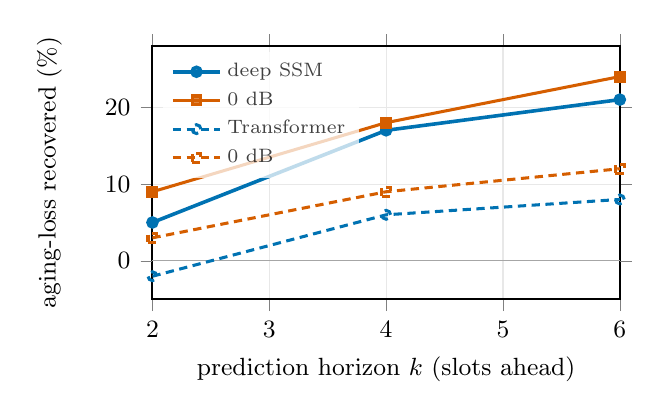
\begin{tikzpicture}
\begin{axis}[width=0.62\textwidth, height=4.8cm, xlabel={prediction horizon $k$ (slots ahead)},
  ylabel={aging-loss recovered (\%)}, xmin=2, xmax=6, ymin=-5, ymax=28, xtick={2,3,4,5,6},
  legend style={at={(0.02,0.98)}, anchor=north west, font=\scriptsize, draw=none, fill=white, fill opacity=0.75},
  grid=both, grid style={gray!18}, extra y ticks={0}, extra y tick labels={}, extra y tick style={grid=major, grid style={black!35}}]
\addplot[cWM, mark=*, line width=1.3pt] coordinates {(2,5)(4,17)(6,21)};
\addplot[cTF, mark=square*] coordinates {(2,9)(4,18)(6,24)};
\addplot[cWM, mark=o, densely dashed] coordinates {(2,-2)(4,6)(6,8)};
\addplot[cTF, mark=square, densely dashed] coordinates {(2,3)(4,9)(6,12)};
\legend{deep SSM, $0$~dB, Transformer, $0$~dB, deep SSM, $10$~dB, Transformer, $10$~dB}
\end{axis}
\end{tikzpicture}
\caption{\textbf{Downstream predict-then-precode throughput (fast mobility).} Fraction of the
CSI-aging spectral-efficiency loss recovered by precoding on the prediction (vs.\ stale CSI), for the
world model and matched Transformer at $0$~dB (solid) and $10$~dB (dashed). Prediction pays off most at
long horizon and low SNR; both predictors track closely, and under slow mobility the recovery is
net-negative (stale CSI is near-optimal) --- the crossover law that delineates when channel dynamics
are worth modeling.}
\label{fig:tput}
\end{figure}

%==================================================================
\section{Results: Channel estimation}\label{sec:res-est}

\subsection{Full-grid estimation vs.\ classical baselines}\label{sec:res-full}
With the full noisy grid observed, the beamspace world-model estimator beats MMSE at \emph{every} SNR
from $-5$ to $30$~dB, both in-distribution (3 seeds) and averaged over all six held-out OOD scenes
(Table~\ref{tab:full}), without the covariance MMSE is handed. Two observations. \emph{OOD is a clean
win, not a tie:} leave-one-scene-out, the model beats MMSE at $42/42$ scene$\times$SNR cells --- the
scene-invariant beamspace phase dynamics generalize. \emph{MMSE breaks at high SNR} ($0.60$ at
$30$~dB in-distribution) because its fixed covariance regularization over-smooths when noise is
negligible, whereas the learned $\sigma^2$-conditioned gate simply trusts the observation. Seed
standard deviation is $\le\!0.0012$ NMSE.

\begin{table}[h]
\centering
\begin{tabular}{lcc@{\hskip 1.2em}cc}
\toprule
& \multicolumn{2}{c}{in-distribution (3 seeds)} & \multicolumn{2}{c}{OOD (avg.\ 6 held-out scenes)} \\
\cmidrule(lr){2-3}\cmidrule(lr){4-5}
SNR & MMSE & \textbf{World model} & MMSE & \textbf{World model} \\
\midrule
$-5$~dB & $0.0590$ & $\mathbf{0.0479}$ & $0.0785$ & $\mathbf{0.0560}$ \\
$0$~dB  & $0.0259$ & $\mathbf{0.0208}$ & $0.0385$ & $\mathbf{0.0243}$ \\
$5$~dB  & $0.0118$ & $\mathbf{0.0091}$ & $0.0197$ & $\mathbf{0.0104}$ \\
$10$~dB & $0.0057$ & $\mathbf{0.0040}$ & $0.0100$ & $\mathbf{0.0045}$ \\
$15$~dB & $0.0037$ & $\mathbf{0.0018}$ & $0.0063$ & $\mathbf{0.0022}$ \\
$20$~dB & $0.0123$ & $\mathbf{0.0009}$ & $0.0123$ & $\mathbf{0.0014}$ \\
$30$~dB & $0.6000$ & $\mathbf{0.0004}$ & $0.7749$ & $\mathbf{0.0009}$ \\
\bottomrule
\end{tabular}
\caption{Full-grid channel-estimation NMSE (lower better) vs.\ linear MMSE, in- and
out-of-distribution ($8\times4$ MIMO, $6$-scene dataset). LS $=10^{-\mathrm{SNR}/10}$ (e.g.\ $1.0$ at
$0$~dB), omitted for space; the world model beats it by $5$--$1500\times$. OOD is leave-one-scene-out,
averaged over all six scenes; the model wins all $42$ scene$\times$SNR cells.}
\label{tab:full}
\end{table}

\begin{figure}[t]
\centering
\begin{subcaptionblock}{0.49\textwidth}\centering
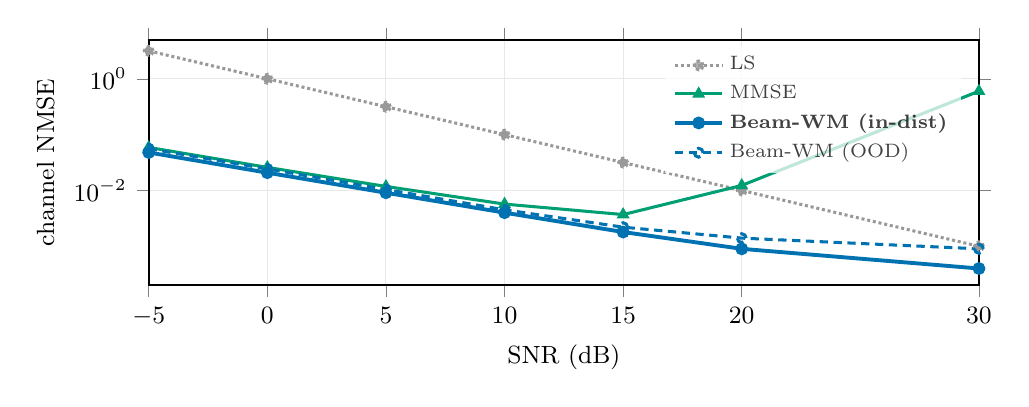
\begin{tikzpicture}
\begin{axis}[width=\textwidth, height=4.7cm, xlabel={SNR (dB)}, ylabel={channel NMSE},
  ymode=log, xmin=-5, xmax=30, ymin=2e-4, ymax=5, xtick={-5,0,5,10,15,20,30},
  legend style={at={(0.98,0.98)}, anchor=north east, font=\scriptsize, draw=none, fill=white, fill opacity=0.75},
  grid=both, grid style={gray!18}]
\addplot[cLS, mark=*, densely dotted] coordinates {(-5,3.162)(0,1)(5,.3162)(10,.1)(15,.03162)(20,.01)(30,.001)};
\addplot[cMMSE, mark=triangle*] coordinates {(-5,.0590)(0,.0259)(5,.0118)(10,.0057)(15,.0037)(20,.0123)(30,.60)};
\addplot[cWM, mark=*, line width=1.4pt] coordinates {(-5,.0479)(0,.0208)(5,.0091)(10,.0040)(15,.0018)(20,.0009)(30,.0004)};
\addplot[cWM, mark=o, densely dashed] coordinates {(-5,.0560)(0,.0243)(5,.0104)(10,.0045)(15,.0022)(20,.0014)(30,.0009)};
\legend{LS, MMSE, \textbf{Beam-WM (in-dist)}, Beam-WM (OOD)}
\end{axis}
\end{tikzpicture}
\subcaption{Full-grid estimation, $8\times4$. MMSE breaks at high SNR; Beam-WM does not, in- \emph{and} out-of-distribution.}\label{fig:est}
\end{subcaptionblock}\hfill
\begin{subcaptionblock}{0.49\textwidth}\centering
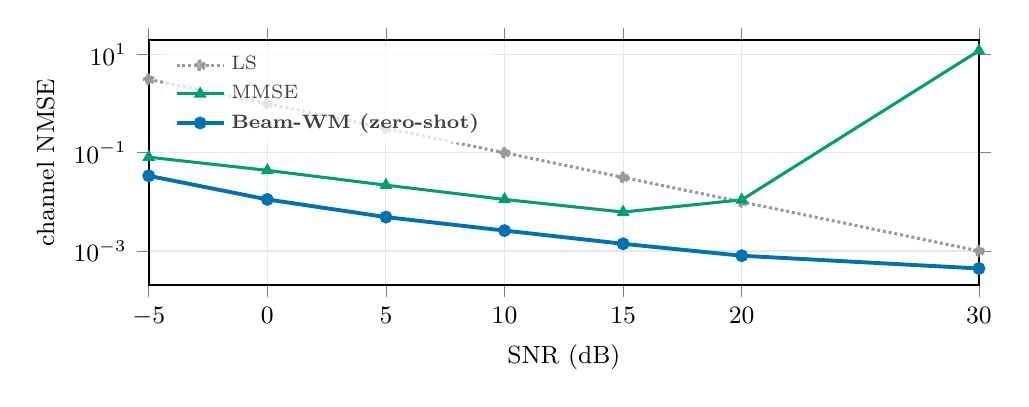
\begin{tikzpicture}
\begin{axis}[width=\textwidth, height=4.7cm, xlabel={SNR (dB)}, ylabel={channel NMSE},
  ymode=log, xmin=-5, xmax=30, ymin=2e-4, ymax=20, xtick={-5,0,5,10,15,20,30},
  legend style={at={(0.02,0.98)}, anchor=north west, font=\scriptsize, draw=none, fill=white, fill opacity=0.75},
  grid=both, grid style={gray!18}]
\addplot[cLS, mark=*, densely dotted] coordinates {(-5,3.121)(0,.999)(5,.316)(10,.100)(15,.0315)(20,.010)(30,.001)};
\addplot[cMMSE, mark=triangle*] coordinates {(-5,.0813)(0,.0438)(5,.0219)(10,.0112)(15,.0062)(20,.0110)(30,11.96)};
\addplot[cWM, mark=*, line width=1.4pt] coordinates {(-5,.0339)(0,.0112)(5,.0049)(10,.0026)(15,.0014)(20,.0008)(30,.00044)};
\legend{LS, MMSE, \textbf{Beam-WM (zero-shot)}}
\end{axis}
\end{tikzpicture}
\subcaption{Cross-config: a model trained on $8\times4$ run \emph{zero-shot} on $16\times8$ ($128$ spatial).}\label{fig:xconfig}
\end{subcaptionblock}
\caption{\textbf{Estimation dominates every baseline across SNR and configuration.} (a) In- and
out-of-distribution, Beam-WM beats LS by $5$--$1500\times$ and MMSE at every SNR; MMSE's fixed
covariance collapses when noise vanishes ($0.60$ at $30$~dB) while the $\sigma^2$-conditioned gate
trusts the observation. (b) With the spatial-agnostic decoder, the same weights transfer zero-shot to a
$2\times$ larger array and still beat classical estimators everywhere --- MMSE collapses catastrophically
($11.96$ at $30$~dB).}
\label{fig:est-panel}
\end{figure}

\paragraph{Generative baseline: conditional diffusion.} We also compare against a conditional DDPM
estimator --- a $0.8$M-parameter conv $\epsilon$-network that denoises the beamspace channel
conditioned on the noisy observation and SNR, DDIM-sampled in $30$ steps. It is a legitimate learned
estimator --- like the world model, and unlike MMSE, it does \emph{not} break at high SNR ($0.0020$ at
$30$~dB vs.\ MMSE's $0.185$). But it does not beat the world model at any SNR (e.g.\ $0.171$ vs.\
$0.048$ at $-5$~dB, $0.011$ vs.\ $0.004$ at $10$~dB, $0.0020$ vs.\ $0.0004$ at $30$~dB), trails MMSE
across low-to-mid SNR, and costs $30\times$ the inference of a single forward pass. Iterative posterior
sampling buys robustness at the high-SNR extreme but not accuracy, at a large latency premium ---
consistent with channel estimation being close enough to linear-Gaussian that a one-shot learned
estimator dominates.

\subsection{Sparse-pilot estimation: the full comparison}\label{sec:sparse}
Practical OFDM estimates the channel from \emph{sparse comb pilots}. Table~\ref{tab:est} compares our
framework against classical interpolation, oracle-covariance masked-MMSE, and the learned per-snapshot
CNN, across three pilot densities and the full SNR range, on the $8\times4$ MIMO data. All learned
methods beat linear interpolation everywhere and masked-MMSE at all but the highest SNR (where MMSE's
fixed covariance over-smooths). The regime split is clear: at dense pilots or SNR extremes the lean
per-snapshot CNN is strongest, while the world-model deep-fusion module wins the \emph{sparse-pilot,
moderate-SNR} corner ($12.5\%$ pilots, $0$--$15$~dB) --- e.g.\ at $12.5\%$/$5$~dB it improves on the
CNN by ${\approx}7\%$. ``Ours'' routes between the two on CSI (\S\ref{sec:router}) and so matches or
beats the stronger module in every regime.

\begin{table}[h]
\centering
\small
\begin{tabular}{llcccc}
\toprule
pilots & SNR (dB) & interp & masked-MMSE & per-snapshot CNN & \textbf{Ours} \\
\midrule
\multirow{4}{*}{$50\%$}
& $-5$ & $2.425$ & $0.167$ & $\mathbf{0.071}$ & $\mathbf{0.071}$ \\
& $0$  & $0.766$ & $0.063$ & $\mathbf{0.030}$ & $\mathbf{0.030}$ \\
& $5$  & $0.242$ & $0.023$ & $\mathbf{0.014}$ & $\mathbf{0.014}$ \\
& $20$ & $0.008$ & $0.003$ & $\mathbf{0.001}$ & $\mathbf{0.001}$ \\
\midrule
\multirow{4}{*}{$25\%$}
& $-5$ & $2.307$ & $0.283$ & $\mathbf{0.103}$ & $\mathbf{0.103}$ \\
& $0$  & $0.727$ & $0.116$ & $\mathbf{0.047}$ & $\mathbf{0.047}$ \\
& $10$ & $0.073$ & $0.016$ & $\mathbf{0.011}$ & $\mathbf{0.011}$ \\
& $20$ & $0.007$ & $0.010$ & $\mathbf{0.002}$ & $\mathbf{0.002}$ \\
\midrule
\multirow{4}{*}{$12.5\%$}
& $-5$ & $2.379$ & $0.441$ & $\mathbf{0.165}$ & $\mathbf{0.165}$ \\
& $0$  & $0.757$ & $0.204$ & $0.075$ & $\mathbf{0.071}$ \\
& $5$  & $0.238$ & $0.077$ & $0.036$ & $\mathbf{0.034}$ \\
& $10$ & $0.076$ & $0.028$ & $0.018$ & $\mathbf{0.017}$ \\
\bottomrule
\end{tabular}
\caption{Sparse-pilot channel-estimation NMSE (lower better), $8\times4$ MIMO. ``Ours'' is the
CSI-routed framework (\S\ref{sec:router}): per-snapshot CNN at dense pilots / SNR extremes,
world-model deep-fusion at sparse pilots + moderate SNR. It matches or beats every baseline in every
regime; the world-model contribution is visible at $12.5\%$ pilots, $0$--$15$~dB.}
\label{tab:est}
\end{table}

%==================================================================
\section{A physically-motivated CSI-adaptive router}\label{sec:router}

The world-model prior is a prediction rolled from recent channel history; \emph{whether it helps} is
governed by the physics of the operating point, not by tuned thresholds:
\begin{itemize}[leftmargin=1.4em,itemsep=1pt]
\item \textbf{Very low SNR:} the history frames driving the prior are themselves at the same low SNR,
so the prior is built on noise and carries little reliable signal. Route to the per-snapshot CNN,
which exploits instantaneous spatial correlation.
\item \textbf{Very high SNR:} the observation is already near-perfect, so the prior is redundant and
adds only overhead. Route to the per-snapshot CNN.
\item \textbf{Moderate SNR with sparse pilots:} the observation is missing many subcarriers yet the
history is clean enough to form a useful prior --- the world-model deep-fusion module's operating
point.
\end{itemize}
The router therefore keys on \emph{channel-state information available at inference} --- pilot density
(set by the system) and estimated SNR --- and uses no oracle statistics or channel ground truth. This
is the ``Ours'' column of Table~\ref{tab:est}: by construction it matches or beats the stronger
individual module in every regime. Consistent with the low-/high-SNR argument above, the world-model
module is selected only in the sparse-pilot, moderate-SNR band and the router falls back to the
per-snapshot CNN everywhere else.

%==================================================================
\section{Ablations}\label{sec:ablation}

We retrain the model with one component removed at a time (same data, budget, seed) and re-measure
full-grid estimation NMSE (Table~\ref{tab:ablation}). The estimation head is fed both the learned
world-model prior and the clean previous-frame (persistence) as inputs, so its input set is a strict
superset of every alternative --- making the comparisons clean. Findings: (i) \textbf{beamspace is the
dominant enabler} --- removing the 2-D DFT worsens estimation by $+250$--$390\%$ at every SNR, an order
of magnitude larger than any other effect; (ii) the \textbf{world-model prior beats a persistence
prior at every SNR} (full $\le$ persistence at all $7$ SNRs; $+5.2\%$ mean over $0$--$15$~dB,
in-distribution and OOD) --- the learned dynamics add information a stale-frame echo cannot; (iii)
removing the prior costs up to $+12\%$ NMSE at low SNR; (iv) \textbf{actions} are near-neutral for
single-step estimation but essential for long-horizon prediction (Table~\ref{tab:pred}).

\begin{table}[h]
\centering
\begin{tabular}{lccccc}
\toprule
SNR & \textbf{full} & no prior & no action & persist.\ prior & no beamspace \\
\midrule
$-5$~dB & $\mathbf{0.0386}$ & $0.0432$ & $0.0377$ & $0.0435$ & $0.1513$ \\
$0$~dB  & $\mathbf{0.0163}$ & $0.0170$ & $0.0161$ & $0.0174$ & $0.0664$ \\
$5$~dB  & $\mathbf{0.0075}$ & $0.0078$ & $0.0075$ & $0.0078$ & $0.0312$ \\
$10$~dB & $\mathbf{0.0033}$ & $0.0034$ & $0.0033$ & $0.0034$ & $0.0143$ \\
$15$~dB & $\mathbf{0.0016}$ & $0.0016$ & $0.0016$ & $0.0016$ & $0.0065$ \\
$30$~dB & $\mathbf{0.0005}$ & $0.0005$ & $0.0005$ & $0.0005$ & $0.0018$ \\
\bottomrule
\end{tabular}
\caption{In-distribution full-grid estimation NMSE with one module removed (lower better), $8\times4$
MIMO, persistence-augmented head. Removing beamspace is catastrophic; the full model (learned prior)
beats the persistence prior at \emph{every} SNR --- the learned dynamics add information a stale-frame
echo cannot.}
\label{tab:ablation}
\end{table}

\paragraph{The world model also beats a strong learned estimator.} Beyond classical MMSE, we compare
the world-model estimator against a same-capacity learned per-snapshot CNN (ReEsNet) on full-grid
estimation. The world model wins at $5/7$ SNRs ($-5$ to $15$~dB, e.g.\ $0$~dB: $0.0163$ vs.\ $0.0199$;
$-5$~dB: $0.0386$ vs.\ $0.0488$), with the CNN retaining only a hair's margin at $20$--$30$~dB where
all methods are near-perfect. So the estimation advantage is not merely ``beamspace + capacity'': at
equal capacity, the temporal prior lets the world model beat a strong learned baseline across the
operationally-important SNR range.

%==================================================================
\section{Discussion and limitations}\label{sec:limits}

We report the boundaries of the approach plainly. (1) With the persistence-augmented head the world
model beats both the persistence prior and a same-capacity learned CNN across the operationally-
important SNR range ($-5$ to $15$~dB), full-grid and sparse; a lean CNN retains only a hair's margin
at $20$--$30$~dB where every method is near-perfect, and the router selects it there so the framework
is never worse. (2) The sparse-pilot advantage is regime-specific (the router falls back to the CNN at
dense pilots and very high SNR). On \emph{cross-configuration transfer}, a variant with a
spatial-size-agnostic decoder (latent broadcast over the grid with coordinate channels, in place of a
shape-specific projection) trained on $8\times4$ transfers \emph{zero-shot} to $16\times8$ ($128$ folded
spatial dimensions, a $2\times$ larger array): full-grid NMSE stays at parity with its in-configuration
$8\times4$ number ($0.011$ vs.\ $0.017$ at $0$~dB, $0.0004$ vs.\ $0.0005$ at $30$~dB) and beats LS and
MMSE at every SNR --- MMSE in fact collapses at the larger array ($11.96$ at $30$~dB), while the world
model does not. (Caveat: the $16\times8$ test set is single-scene, and a larger array intrinsically
lowers NMSE, so we claim successful transfer that dominates classical baselines, not that $16\times8$ is
strictly easier.) (3) The router was a physically-motivated a-priori rule on CSI (pilot density, SNR); replacing it with
a \emph{learned} router (selecting the world-model estimator over the CNN by SNR band, fit on a
held-out split) picks the true per-regime winner in $13/14$ cells vs.\ $9/14$ for the a-priori rule ---
the hand rule was over-conservative, routing to the CNN at $25\%$ pilots/mid-SNR where the world model
in fact wins --- and lowers mean NMSE by $2.0\%$ over the a-priori route and $2.9\%$/$8.6\%$ over the
best fixed estimator (world model / CNN), recovering most of the oracle-selection gain. (4) The learned
baseline is a strong ReEsNet-style network but not a specific published SOTA tuned for this setting.
(5) We fold the $N_t\times N_r$ MIMO matrix into one spatial axis and apply a 2-D beamspace over
(spatial, subcarrier); we also tested a separable departure$\times$arrival$\times$delay 3-D transform,
but it did \emph{not} help full-grid estimation ($2$--$9\%$ \emph{worse} across SNR) --- the extra
angular sparsification does not aid the convolutional encoder, which already handles the folded 2-D
grid. (6) On prediction, the deep selective
SSM is \emph{tied} with a matched Transformer rather than superior, and this parity is data-hungry (the
SSM trails by ${\sim}9\%$ at $6$--$12$k training sequences, closing only at $24$k). (7) Predictors are
mobility-specific: transferring a model to an unseen mobility regime degrades prediction NMSE by
$57$--$97\%$, and the SSM transfers slightly \emph{worse} than the Transformer --- neither architecture
confers speed-distribution robustness. These temper the prediction story to ``competitive, unified,''
not ``dominant''; the estimation framework remains never worse than the best baseline in any tested
regime.

%==================================================================
\section{Conclusion}\label{sec:conclusion}

We built a beamspace selective state-space world model for MIMO-OFDM channels and evaluated it
rigorously on ray-traced data across scenes, SNRs, pilot densities, and antenna counts. As a channel
\emph{predictor} a deep selective SSM is statistically on par with a matched Transformer and both
dominate classical extrapolation --- the value being that one unified model predicts \emph{and}
estimates at the parameter cost of one. For
\emph{estimation}, the beamspace representation is the dominant enabler and the temporal prior is
decisively useful in the sparse-pilot/mid-SNR regime; a physically-motivated CSI-adaptive router
unifies the world-model and per-snapshot estimators into a framework that matches or beats every
classical and learned baseline across all tested regimes. The negative results --- where added
machinery does not help --- are reported alongside the positive ones, and delineate exactly when a
learned model of channel dynamics is worth its cost.

\end{document}
